\documentclass[
headings=optiontohead,              % allows double headers
12pt,                               % fontsize 
DIV=13,                             % koma script diveider amount. tells koma how much of the site can be written to
twoside=false,                      % if set to true, automatically formats as book style with different left and right pages
open=right,                         % starting page on twosided texts 
BCOR=10mm,                          % correction that accounts for the center of the pages being glued in
toc=bibliographynumbered            % bibliography gets a number and is listed in the table of contents
]{scrreport}

\usepackage[utf8]{inputenc}                     % correct encoding of output, technically not needed anymore
\usepackage[T1]{fontenc}                        % correct encoding of output, technically not needed anymore
\usepackage[english]{babel}                     % font that supports English
\usepackage{upgreek}                            % non-cursive Greek letters
\usepackage[stretch=10,shrink=10,protrusion=true,expansion=true,final]{microtype} % prettier block format
\usepackage{hyperref}                           % links for everything
\usepackage{color}                              % allows for setting in different colors
\usepackage[autooneside=false,automark]{scrlayer-scrpage} % page-style with "Kolumnentitel" (title of current chapter is displayed at the top)
\usepackage{lmodern}                            % alternative font (better use libertinus)
\usepackage[sb]{libertinus}                     % use the font libertinus (needs to be installed from the web)
\usepackage[slantedGreek]{libertinust1math}     % math mode improvement for libertinus
\usepackage{siunitx}                            % physical units setting
\usepackage{icomma}                             % commas in lists get extra space if needed                        
\usepackage{amsfonts,amssymb,amstext,amsmath,amsthm} % better math mode (\mathrm and \text) and symbols
\usepackage{xspace}                             % works to improve own commands and provides "\xspace"-command, that puts a space if needed
\usepackage{ifthen}                             % more control over non-obligatory parameters
\usepackage{titling}                            % get title values as macros
\usepackage[onehalfspacing]{setspace}           % control the spacing between lines and in enumeration lists
\usepackage[backend=biber, style=phys, biblabel=brackets]{biblatex} % citations with "modern" backend and an physics-accepted citation style
\usepackage{graphicx}                           % work with graphics 
\usepackage{ragged2e}                           % ragged-commands (when no block format is wanted)
\usepackage{pdfpages}                           % allows including of pdfs into this pdf
\usepackage{booktabs}                           % better table formatting
\usepackage{multicol}                           % allows for the definition of multi-columns in tables
\usepackage{multirow}                           % allows for the definition of multirow-tables instead of just multicolumn
\usepackage[section]{placeins}                  % provides the command "\FloatBarrier" to control the end of floatable regions for figures/tables
\usepackage{float}                              % provides the "H" option for forcing placement of a figure
\usepackage{floatpag}                           % make it possible for float-pages to not have a page number
\usepackage{url}                                % sometimes needed by biblatex, technically no longer needed
\usepackage{minted}                             % nice code highlighting (needs Python Package to compile!!)
\usepackage{accents}                            % better control over accents
\usepackage{mathtools}                          % more math control possibilities
\usepackage[autostyle=true]{csquotes}           % context-sensitive-quotes -> quotation marks that are set correctly for the context
\usepackage{physics}                            % bra-ket and more
\usepackage{nicematrix}                         % label row/cols on matrix
\usepackage{caption}                            % caption of different envoironments

\title{Investigation of transformer architectures for geometrical graph structures and their application to two-dimensional spin systems} % TODO lookup title
\author{Jonas Kell}
\date{7$^\text{th}$ October 2022}

\graphicspath{{./images/}}              % custom paths for folders in that graphics can be found

\sisetup                                % setup for siunitx
{
detect-all,
locale=US,                              % language setup for siunitx
range-phrase={ \text{to} },             % word that is put into an si range
range-units = single,                 % better display of error ranges
per-mode=symbol-or-fraction,            % more dynamic frac usage in inline/displaymath mode
separate-uncertainty,                   % for better +- , \pm when including an error range 
}

\hypersetup
{
colorlinks=true,
linkcolor=dblue,                                    % dark blue linkcolor
urlcolor=dblue,                                     % dark blue linkcolor
citecolor=dblue,                                    % dark blue linkcolor
pdfauthor = {REDACTED},                           % write details into the expanded file properties
pdftitle = {Investigation of transformer architectures for geometrical graph structures},                         
pdfkeywords = {neural networks, graphs, ai, physics, quantum mechanics, transformers, machine learning},           
pdfsubject = {Bachelor Thesis}                      
}

\AtBeginDocument{
	\let\mathbb\relax
	\DeclareMathAlphabet\PazoBB{U}{fplmbb}{m}{n}
	\newcommand{\mathbb}{\PazoBB}
}       %more options to the \mathbb command

\setminted[]{
    xleftmargin=0cm,
    xrightmargin=0cm,
    frame=single,
    framesep=.25cm,
    linenos,
    tabsize=2,
    breaklines,
    breakafter=.],
    breakaftersymbolpre= ,
}           %configure the minted code-highlighting style

\addbibresource{literature.bib}              %initialize bibtex with correct file

\NiceMatrixOptions{
code-for-first-row = \color{dblue} ,
code-for-last-row = \color{dblue} ,
code-for-first-col = \color{dblue} ,
code-for-last-col = \color{dblue}
}
                                  % another file that holds the package/document configuration
\linespread{1.1}                                    % line-spacing can be controlled here

\clubpenalty10000                                   % Schusterjunge, orphan
\widowpenalty10000                                  % Hurenkind, Witwe
\displaywidowpenalty=10000                          % Make document obey stricter rules considering "Schusterjungen" and "Hurenkinder"
\renewcommand{\topfraction}{0.8}                    % allows for more chilled "text to image ratio" 
\renewcommand{\bottomfraction}{0.8}
\renewcommand{\textfraction}{0.1}
\renewcommand{\floatpagefraction}{0.8}

% \renewcaptionname{ngerman}{\figurename}{Abb.}       %"Figure" becomes "Fig." in English
\setcapindent{0cm}                                  %useful if image captions have multiple lines. Removers indentation below "Fig."
\setlength{\parindent}{0cm}                         %removes indentation at start of new paragraphs


%bibliography slots are redefined/modified here
\DeclareFieldFormat{journaltitle}{\textsl{#1}\isdot}
\DeclareFieldFormat{titlecase}{{#1}}


%COLORS
\definecolor{dblue}{rgb}{0,0,0.5}
\definecolor{dred}{rgb}{0.5,0,0}
\definecolor{dgrey}{rgb}{0.5,0.5,0.5}

%overwrite the coma-script definitions
\addtokomafont{pagehead}{\normalfont\color{dgrey}}                  %overwrite the coma-script definitions
\addtokomafont{sectioning}{\rmfamily\color{dblue}\boldmath}         %rmfamily puts headings in "normal" "serif-font" instead of "sans-serif"  boldmath ensures a bold math font in subscripts
\addtokomafont{captionlabel}{\bfseries\footnotesize}                %better Fig. format
\addtokomafont{caption}{\footnotesize}                          

%! hyphenation commonly used words can be spelled here to provide latex with the correct places to make line breaks
\hyphenation{Li-pid-mono-lage}

% headline spacing
\RedeclareSectionCommand[beforeskip=0cm,afterskip=1cm]{chapter}                                  % another file that holds format information
%! Ref-Commands 
\newcommand*{\fullref}[1]{\hyperref[{#1}]{\textit{\autoref*{#1} \nameref*{#1}}}}
\newcommand*{\fullpage}[1]{\hyperref[{#1}]{Seite \pageref*{#1}}}
\newcommand*{\fullpages}[1]{\hyperref[{#1}]{Seiten \pageref*{#1}ff}}

%! Math operators and other small conveniences
\newcommand\thickbar[1]{\accentset{\rule{.6em}{.8pt}}{#1}}
\DeclareMathOperator{\ggt}{ggT}
\DeclareMathOperator{\kgv}{kgV}
\DeclarePairedDelimiter\ceil{\lceil}{\rceil}
\DeclarePairedDelimiter\floor{\lfloor}{\rfloor}
\renewcommand*{\arraystretch}{0.8}

%! qm commands
\newcommand{\hamiltonian}{\ensuremath{\mathcal{H}}\xspace}
\newcommand{\up}{\ensuremath{\uparrow}\xspace}
\newcommand{\down}{\ensuremath{\downarrow}\xspace}
                                % another file that holds predefined commands


\begin{document}

% ! Bibliography, page numbering and Title setups
\thispagestyle{empty}                           % make sure title page is not numbered or anything else


\newcommand{\mail}{REDACTED}



\begin{titlepage}
\makebox[\textwidth][c]{
\includegraphics[width=0.5\textwidth]{logo_uni_augsburg.jpg}}
    
\color{dblue}

\begin{center}
    \vspace*{2cm}
    \Huge
    \textbf{\thetitle}

    \vspace*{1.5cm}
    \color{black}
    \textbf{Bachelor Thesis}

    \vspace*{1cm}
    \normalsize
    submitted by\\
    \LARGE
    \theauthor\\\vspace*{0.3cm}
    \normalsize
    on \thedate

    \vspace{1.8cm}
    \color{black}
    \emph{Augsburg University}\\
    \emph{Faculty of Applied Computer Science}\\
    \emph{Institute of Computer Science}\\
    \emph{Chair for Machine Learning \& Computer Vision}

    \vfill

    \begin{tabular}{rl}
        1$^\text{st}$ Corrector: &REDACTED\\
        2$^\text{nd}$ Corrector: &REDACTED\\
    \end{tabular}
\end{center}

\end{titlepage}
                               % include title-page
\cleardoublepage                                % make sure, that if double-page is active, to reset the double page counter
\pagestyle{scrheadings}                         % puts current chapters title into the header in small gray font
\pagenumbering{roman}                           % number the pages of the table of contents in roman numerals
\renewcommand{\contentsname}{Table of Contents} % title of table of contents
\tableofcontents                                % table of contents
\noindent\\\\

\addsec*{List of Abbreviations}
\begin{tabular}[h]{p{3cm}|l}
	Abbreviation & Meaning\\
	\hline
	NQS & Neural Quantum State\\
	VMC & Variational Monte Carlo\\
	DMC & Diffusion Monte Carlo\\
	nn & nearest neighbor\\
	nnn & next nearest neighbor\\
	sgd & stochastic gradient descent\\
	GPU & graphics processing unit\\
	ReLU & rectifier linear unit\\
	RBM & restricted Boltzmann machine\\
	fcl & fully connected layer\\
\end{tabular}
\newpage                                   % list of abbreviations, figures, etc
\cleardoublepage                                % make sure, that if double-page is active, to reset the double page counter
\pagenumbering{arabic}                          % number the pages of the main document in Arabic numerals

% After this, the redefinition of the "Kolumnentitel" takes place
\clearpairofpagestyles
\ihead{\leftmark}
\ohead{\Ifstr{\leftmark}{\rightmark}{}{\rightmark}}
\cfoot*{\pagemark}
% End of the "Kolumnentitel" redefinition


% ! Main Document Body
\chapter{Introduction}
\label{sec:introduction}
The first set of experiments will be on the image classification task.
The goal will be to compare the architectural advantages and drawbacks between multiple different kinds of metaformers.

Training was be performed on a subset of 100 classes from the \emph{ImageNet} dataset \cite{imagenetDataset}.
The accompanying code to replicate these experiments can be found on GitHub \cite{selfComputerScience}.

The neural networks, as well as the training and evaluation code were written in python.
The \emph{PyTorch} \cite{pytorchGithub} machine learning framework was used as a measure to efficiently define neural networks and lever the computational capabilities of parallelization via GPUs.

The main metaformer model was originally based on the vision transformer found in an implementation of \emph{DINO} \cite{dinoGithub}, was however heavily modified. 
A comparison between the stock DINO model and the modified version will be also performed.
This however is not supposed to be a direct discrediting of any of the models, as their main purposes do not exactly align.
Therefore one or the other may excel in specific tasks.
Also a comparison against a pre-implemented \emph{poolformer} \cite{poolformerGithub} will be performed.

The \emph{einops} package \cite{einopsGithub} is heavily used. It provides tensor operations, configurable with the \emph{Einstein notation} and simplifies the notation and subsequently readability.
Lastly, the implementation of the \emph{positional encoding} is provided by \cite{positionalEncodingGithub}.

\FloatBarrier
\chapter{Theory}
\label{sec:theory}
    \section{From the Point of Physics}
        \label{sec:theory-physics}
        The first set of experiments will be on the image classification task.
The goal will be to compare the architectural advantages and drawbacks between multiple different kinds of metaformers.

Training was be performed on a subset of 100 classes from the \emph{ImageNet} dataset \cite{imagenetDataset}.
The accompanying code to replicate these experiments can be found on GitHub \cite{selfComputerScience}.

The neural networks, as well as the training and evaluation code were written in python.
The \emph{PyTorch} \cite{pytorchGithub} machine learning framework was used as a measure to efficiently define neural networks and lever the computational capabilities of parallelization via GPUs.

The main metaformer model was originally based on the vision transformer found in an implementation of \emph{DINO} \cite{dinoGithub}, was however heavily modified. 
A comparison between the stock DINO model and the modified version will be also performed.
This however is not supposed to be a direct discrediting of any of the models, as their main purposes do not exactly align.
Therefore one or the other may excel in specific tasks.
Also a comparison against a pre-implemented \emph{poolformer} \cite{poolformerGithub} will be performed.

The \emph{einops} package \cite{einopsGithub} is heavily used. It provides tensor operations, configurable with the \emph{Einstein notation} and simplifies the notation and subsequently readability.
Lastly, the implementation of the \emph{positional encoding} is provided by \cite{positionalEncodingGithub}.

        \FloatBarrier
        \subsection{The Ground State Search}
        \label{sec:theory-groundstatesearch}
        This section is supposed to introduce the fundamentals of (many body) quantum physics.


        \subsection{The Ising Model}
        \label{sec:theory-ising}
        In this thesis, a special case of quantum system will be discussed. 
The \emph{Ising model}.
The model describes multiple \emph{spins} that are locked in place. 
A spin is a very special kind of angular momentum that is inherent to quantum mechanical particles.
It helps to imagine the spin as a tiny magnet, that is locked in place, but can freely rotate to react to to external/neighboring  magnetic fields. This is a very harsh oversimplification, but enough for our purposes.

The state of the \emph{many body wavefunction} can solely be described by the direction that each of the spins is pointing into. In this simplified case, only \emph{spin-$\frac{1}{2}$} particles are used. That means each spin at each position can only either be pointing \emph{up} \up or \emph{down} \down (in relation to the z-axis).

That means, that a system with $n=3$ spins (in arbitrary, but fixed position) can be represented like \ref{eq:spin-ising}. $\vec{s}_m$ is the direction of the spin vector, that can (in this case) be simplified to the z-axis contribution $s^z_m$ of the vector. The values con only be $\frac{1}{2}$ (\up) or $-\frac{1}{2}$ (\down).
In this case the spins at the positions 1 and 2 point up, the one at 3 points down.

\begin{equation}
    \label{eq:spin-ising}
    \ket{\vec{s}_1, \vec{s}_2, \vec{s}_3} \rightarrow \ket{s^z_{1}, s^z_{2}, s^z_{3}} = \ket{\tfrac{1}{2}, \tfrac{1}{2}, -\tfrac{1}{2}} = \ket{\up, \up, \down}
\end{equation}

The hamiltonian for the system is defined as \ref{eq:hamiltonian-ising}. $J_{i, j}$ is the \emph{coupling constant} between the lattice sites $i$ and $j$. $h_i$ is a measure for the external magnetic field (in x-direction) at the lattice site $i$. Often the terms each get multiplied with $-1$ (sing flip of $J$ and $h$) as per convention. This was not done in this case in order for the equation to reflect the code. The $\hat{s}^a_i$ are \emph{operators}, that measure the $s^a_i$ number of the wavefunction (possibly altering its state in the process).

\begin{equation}
    \label{eq:hamiltonian-ising}
    \hamiltonian = \sum\limits_{i, j} J_{i, j} \cdot \hat{s}^z_i \hat{s}^z_j + \sum\limits_{i} h_i \cdot \hat{s}^x_i
\end{equation}

\ref{eq:hamiltonian-ising-nn} is a simplification, that assumes homogeneous interaction constants $J$ and $h$ for all sites, as well as only allowing nearest neighbors ($\langle i, j\rangle$) to interact.

\begin{equation}
    \label{eq:hamiltonian-ising-nn}
    \hamiltonian =  J \cdot \sum\limits_{\langle i, j \rangle} \hat{s}^z_i \hat{s}^z_j + h \cdot \sum\limits_{i} \hat{s}^x_i
\end{equation}

In this form, a $J < 0$ leads to so-called \emph{ferromagnetic} interaction. With a $J > 0$ the interaction is called \emph{anti-ferromagnetic}. When $h \neq 0$, the model is called \emph{transverse field Ising model} \cite{isingBook}.

The model was first solved for a 1D chain by Ernst Ising in 1924 \cite*[]{isingFerromagnetismn}. He solved the ferromagnetic case without a transverse field (however with an additional field parallel to the z-direction). His solution was analytically derived, but already not trivial to come up with.
With the introduction of a transverse field and a more complex lattice structure than a linear chain, there doesn't exist an analytic solution to even the most simplified hamiltonian \ref{eq:hamiltonian-ising-nn}.

In order to be able to use the hamiltonian, a few rules about the interaction of the used operators and the wavefunction will be introduced. They represent only a small subset of the mathematics and focus only on the bare minimum needed to understand the problem as someone that is unfamiliar with quantum mechanics. 

The spin operators can be written in terms of the \emph{Pauli spin matrices} \cite{schwablQM}. This is only mentioned, because it reflects the implementation in the code. Note that in the code, the $\frac{1}{2}$ factors in \ref{eq:pauli-rules} are omitted for simplification. $i$ stands for the complex unit.

\begin{equation}
    \label{eq:pauli-rules}
    \hat{s}^x = \frac{1}{2} \cdot \sigma^x = \frac{1}{2} \cdot \left(\begin{matrix}
        0& 1 \\
        1& 0
    \end{matrix}\right) \quad
    \hat{s}^y = \frac{1}{2} \cdot \sigma^y = \frac{1}{2} \cdot \left(\begin{matrix}
        0& -i \\
        i& 0
    \end{matrix}\right) \quad
    \hat{s}^z = \frac{1}{2} \cdot \sigma^z = \frac{1}{2} \cdot \left(\begin{matrix}
        1& 0 \\
        0& -1
    \end{matrix}\right)
\end{equation}

With the corresponding Pauli representation of the spin vectors \ref{eq:pauli-vectors}, the interaction of the operators can be directly computed with standard matrix multiplication. The important ones are calculated in \ref{eq:pauli-transformation}.

\begin{equation}
    \label{eq:pauli-vectors}
    \ket{\up} = \left(\begin{matrix}
        1\\0
    \end{matrix}\right)
    \qquad
    \ket{\down} = \left(\begin{matrix}
        0\\1
    \end{matrix}\right)
\end{equation}


\begin{equation}
    \label{eq:pauli-transformation}
    \sigma^z \ket{\up} = +1 \cdot \ket{\up} \quad
    \sigma^z \ket{\down} = -1 \cdot \ket{\down} \quad
    \sigma^x \ket{\up} = +1 \cdot \ket{\down} \quad
    \sigma^x \ket{\down} = +1 \cdot \ket{\up}
\end{equation}

The last important piece of information is, that operators denoted by indices only interact with the spin at the corresponding lattice site. Three examples are given in \ref{eq:pauli-many-body}. Multiple operators acting on one state can be computed by only evaluating the effect of the rightmost operator according to the mentioned rules and then repeating until finished. Complex numbers can always be commutatively swapped with operators and bra-kets.

\begin{equation}
    \label{eq:pauli-many-body}
    \sigma^z_2 \ket{\down, \up, \down} = +1 \cdot \ket{\down, \up, \down} \quad
    \sigma^z_1 \ket{\down, \up, \down} = -1 \cdot \ket{\down, \up, \down} \quad
    \sigma^z_3 \ket{\down, \down, \down} = +1 \cdot \ket{\down, \down, \up}
\end{equation}  
        \FloatBarrier
        \subsection{Numerical Solution}
        \label{sec:theory-numericalsolution}
        With the combined knowledge of the two last sections, the ground state (and the ground state energy) can be calculated. On the one hand it will become evident, that the calculation is really simple to do and program. On the other hand it will be shown that it is not feasable to compute sufficiently large lattices, because of the exponential nature of the problem.

\begin{figure}[htbp]
    \centering
    \makebox[\textwidth][c]{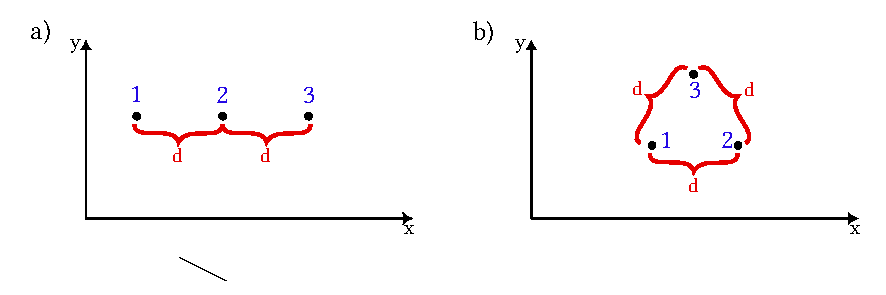
\includegraphics[width=0.9\textwidth]{./theory/physics/numerical-solutions/simple_case.pdf}}
    \vspace{-1cm}
    \caption{A representation of two simple latices. The spins are fixed at the point of the numbered locations. All sites have the same distance $d$ from their neighbors. Note, that a spin up \up is directed parallel to the z-axis. That means in this case it would point out of the paper in the direction of the viewer.}
    \label{fig:simpleThreeLatticeIsing}
\end{figure}

In the beginning one trivial example will be discussed. The lattice is visualized in \autoref{fig:simpleThreeLatticeIsing}a.
This corresponds to a linear lattice in 1D. Let the hamiltonian be the one in \autoref{eq:hamiltonianExampleA}.

\begin{equation}
    \label{eq:hamiltonianExampleA}
    \hamiltonian = \sigma^z_1\sigma^z_2 + \sigma^z_2\sigma^z_3
\end{equation}

This hamiltonian is anti-ferromagnetic ($J = +1$), therefore the energy $E$ in \autoref{eq:schroedinger-general} becomes minimal (largest magnitude with negative sign) when the spins always point into the opposite direction as their neighbors: $\ket{\up, \down, \up}$ or $\ket{\down, \up, \down}$. This is quite a crucial step, so validating this yourself is advised for someone without prior quantum mechanical experience.
The ground state therefore will be a \emph{superposition} consisting of equal parts $\ket{\up, \down, \up}$ and $\ket{\down, \up, \down}$ (\autoref{eq:solutionSimpleExample}). The factor $\frac{1}{\sqrt[]{2}}$ instead of the seemingly more obvious $\frac{1}{2}$ makes the wavefunction be \emph{normalized}. If it wasn't for the square root, \autoref{eq:base-orthonormal} would not be satisfied. This way it is satisfied, which can be tested.

\begin{equation}
    \label{eq:solutionSimpleExample}
    \ket{\Psi_\mathrm{gnd}} = \frac{1}{\sqrt[]{2}} \cdot \ket{\up, \down, \up} +  \frac{1}{\sqrt[]{2}} \cdot \ket{\down, \up, \down}
\end{equation}

The second example, visualized in \autoref{fig:simpleThreeLatticeIsing}b, however is not as simple. The corresponding hamiltonian can be seen in \autoref{eq:hamiltonianExampleB}.
\begin{equation}
    \label{eq:hamiltonianExampleB}
    \hamiltonian = \sigma^z_1\sigma^z_2 +\sigma^z_2\sigma^z_3 +\sigma^z_1\sigma^z_3
\end{equation}
It has one more interaction than the previous one. Even though it also is anti-symmetric, it is \emph{not} possible to align all three spins in a way, so that they stand anti-parallel to all their neighbors. This phenomenon is called \emph{frustration} \cite{frustration}.

Already this minimal problem has a complex superposition of eight base states as a ground state. The introduction of the transverse field will only make this more complex. Therefore a systematic way of finding the solution will be presented.

For this purpose, the example from \autoref{fig:simpleThreeLatticeIsing}b will be used once more, but this time with the hamiltonian in \autoref{eq:hamiltonianExampleTransverse}.
\begin{equation}
    \label{eq:hamiltonianExampleTransverse}
    \hamiltonian = J\cdot \sigma^z_1\sigma^z_2 +J\cdot\sigma^z_2\sigma^z_3 +J\cdot\sigma^z_1\sigma^z_3
    +h \sigma^x_1+h \sigma^x_2+h \sigma^x_3
\end{equation}

The goal is now, to write the hamiltonian \hamiltonian as a matrix. 
The elements of the matrix should be $\bra{m}\hamiltonian\ket{n}$. Where $\ket{m}$ and $\ket{n}$ are two states out of the chosen basis. In this case the eight base states are the following (\emph{canonical spin basis}):

\begin{center}
    \begin{tabular}{llll} 
        1: $\ket{\up, \up, \up}$ & 2: $\ket{\up, \up, \down}$  & 3: $\ket{\up, \down, \up}$  & 4: $\ket{\up, \down, \down}$ \\
        5: $\ket{\down, \up, \up}$ & 6: $\ket{\down, \up, \down}$  & 7: $\ket{\down, \down, \up}$  & 8: $\ket{\down, \down, \down}$ 
    \end{tabular}
\end{center}

In \autoref{eq:matrixElement} an example calculation of $\bra{2}\hamiltonian\ket{4}$ is presented.

\begin{equation}
    \label{eq:matrixElement}
    \begin{split}
        &\bra{\up, \up, \down} \hamiltonian \ket{\up, \down, \down} = \\\\ % new line
         \bra{\up, \up, \down} J\cdot \sigma^z_1\sigma^z_2 \ket{\up, \down, \down} +
         &\bra{\up, \up, \down} J\cdot \sigma^z_2\sigma^z_3 \ket{\up, \down, \down} +
         \bra{\up, \up, \down} J\cdot \sigma^z_1\sigma^z_3 \ket{\up, \down, \down} +\\
         \bra{\up, \up, \down} h\cdot \sigma^x_1 \ket{\up, \down, \down} +
         &\bra{\up, \up, \down} h\cdot \sigma^x_2 \ket{\up, \down, \down} +
         \bra{\up, \up, \down} h\cdot \sigma^x_3 \ket{\up, \down, \down}\stackrel{\ref{eq:pauli-transformation}, \ref{eq:pauli-many-body}}{=}\\\\ % new line
          \bra{\up, \up, \down} J\cdot  1 \cdot (-1) \ket{\up, \down, \down} +
         & \bra{\up, \up, \down} J\cdot (-1) \cdot (-1) \ket{\up, \down, \down} +
          \bra{\up, \up, \down} J\cdot  1 \cdot (-1) \ket{\up, \down, \down} +\\
          \bra{\up, \up, \down} h\cdot  1 \cdot \ket{\down, \down, \down} +
         & \bra{\up, \up, \down} h\cdot 1 \cdot \ket{\up, \up, \down} +
          \bra{\up, \up, \down} h\cdot  1 \cdot \ket{\up, \down, \up} =\\\\ % new line
          (-J)\cdot      \bra{\up, \up, \down}  \ket{\up, \down, \down} +
         & J\cdot        \bra{\up, \up, \down} \ket{\up, \down, \down} +
          (-J)\cdot      \bra{\up, \up, \down}  \ket{\up, \down, \down} +\\
          h\cdot         \bra{\up, \up, \down}  \ket{\down, \down, \down} +
         & h\cdot        \bra{\up, \up, \down} \ket{\up, \up, \down} +
          h\cdot         \bra{\up, \up, \down}  \ket{\up, \down, \up}\stackrel{\ref{eq:base-orthonormal}}{=}\\\\ % new line
          (-J)\cdot 0 + J\cdot 0 &+  (-J)\cdot 0 + h\cdot 0  + h\cdot 1 + h\cdot 0   = h 
    \end{split}
\end{equation}

Placing them inside a matrix at the corresponding location yields the matrix representation for $\bra{m}\hamiltonian\ket{n}$ that can be seen in \autoref{eq:matrix-hamiltonian}.
Because of \autoref{eq:base-factors}, each wavefunction can be written in terms of the chosen base. This is used in \autoref{eq:matrix-hamiltonian-vector}. By representing the wavefunction as a column vector, filled with the scaling factors, the transformation is complete. 
The calculation of the hamiltonian \hamiltonian acting on a wavefunction $\Psi$ as in \autoref{eq:schroedinger-general} can now be computed analogously by performing the matrix multiplication $\bra{m}\hamiltonian\ket{n} \cdot \Psi_\mathrm{vec}$.

\begin{equation}
    \label{eq:matrix-hamiltonian}
    \begin{pNiceMatrix}[first-row,first-col]
        &
        \ket{\up, \up, \up}&
        \ket{\up, \up, \down}&
        \ket{\up, \down, \up}&
        \ket{\up, \down, \down}&
        \ket{\down, \up, \up}&
        \ket{\down, \up, \down}&
        \ket{\down, \down, \up}&
        \ket{\down, \down, \down}\\
        \bra{\up, \up, \up}        \phantom{.} & 3 \cdot J  & h         & h         & 0         & h         & 0         & 0         & 0   \\
        \bra{\up, \up, \down}      \phantom{.} & h          &-1 \cdot J & 0         & h         & 0         & h         & 0         & 0   \\
        \bra{\up, \down, \up}      \phantom{.} & h          & 0         &-1 \cdot J & h         & 0         & 0         & h         & 0   \\
        \bra{\up, \down, \down}    \phantom{.} & 0          & h         & h         &-1 \cdot J & 0         & 0         & 0         & h   \\
        \bra{\down, \up, \up}      \phantom{.} & h          & 0         & 0         & 0         &-1 \cdot J & h         & h         & 0   \\
        \bra{\down, \up, \down}    \phantom{.} & 0          & h         & 0         & 0         & h         &-1 \cdot J & 0         & h   \\
        \bra{\down, \down, \up}    \phantom{.} & 0          & 0         & h         & 0         & h         & 0         &-1 \cdot J & h   \\
        \bra{\down, \down, \down}  \phantom{.} & 0          & 0         & 0         & h         & 0         & h         & h         & 3 \cdot J \\
    \end{pNiceMatrix}
\end{equation}

\begin{equation*}
    \begin{split}
        \Psi = 
            &c_1 \ket{\up, \up, \up}  +
            c_2 \ket{\up, \up, \down}  +
            c_3 \ket{\up, \down, \up}  +
            c_4 \ket{\up, \down, \down}  +\\
            &c_5 \ket{\down, \up, \up} +
            c_6 \ket{\down, \up, \down}  +
            c_7 \ket{\down, \down, \up}  +
            c_8 \ket{\down, \down, \down}
    \end{split}
\end{equation*}
\begin{equation} % this is very bad style, but it would not for the life me let this stuff be aligned properly
    \label{eq:matrix-hamiltonian-vector}        
    \longrightarrow\\
\end{equation}
\begin{equation*}
    \begin{split}
        \Psi_\mathrm{vec} = 
        \begin{pNiceMatrix}[first-row]
            \ket{\up, \up, \up}&
            \ket{\up, \up, \down}&
            \ket{\up, \down, \up}&
            \ket{\up, \down, \down}&
            \ket{\down, \up, \up}&
            \ket{\down, \up, \down}&
            \ket{\down, \down, \up}&
            \ket{\down, \down, \down}\\
            c_1&   
            c_2&
            c_3&
            c_4&
            c_5&
            c_6&
            c_7&
            c_8
        \end{pNiceMatrix} \raisebox{0.7em}{T}
    \end{split}
\end{equation*}

Rewriting \autoref{eq:schroedinger-general} in terms of the newly defined matrix operators, results in \autoref{eq:schroedinger-matrix}.
\begin{equation}
    \label{eq:schroedinger-matrix}
    \bra{m}\hamiltonian\ket{n} \cdot \Psi_\mathrm{vec} = E \cdot \Psi_\mathrm{vec}
\end{equation}

This representation is quite useful, because now the problem of finding the eigenstates has been turned into a problem of finding the eigenvectors for a sparse (hermitian) matrix. 
A problem, that is already solved by a lot of algorithms and software \cite{scipyeigsh}.
It is now clear, that the smallest eigenvalue of the matrix \emph{is} the ground state energy and the corresponding eigenvector \emph{is} a representation for the ground state wavefunction.

As mentioned, the complexity of the problem does not lie in terms of how to compute this value, but in how to compute it in reasonable time.
If $L$ is the size of the lattice, it is obvious, that the canonical base contains $2^L$ states ($L$ sites, each can be \up or \down).
Therefore the matrix whose eigenvalues are required has $2^{2\cdot L}$ entries, of which $2^L \cdot m$ are non-zero ($m$ being constant and dependent on the form of the hamiltonian, as well as the number of neighbors to one site in the lattice). 

So even \emph{if} a algorithm was found, to compute the eigenvalues of such a matrix in linear time (in comparison to the number of non-zero entries in the matrix), the time complexity for solving the problem would still scale in $\mathcal{O} (2^L)$ with the number of lattice sites $L$.

To compute macroscopic crystals, the number of lattice sites would have to be in the same range of magnitude as \emph{Avogadros constant} ($N_\mathrm{A} \approx \SI{6.022E23}{\per\mol}$ \cite{avogadrosNumber}). Current hardware can not go reasonably into the range of hundreds. 

This naive algorithm is implemented in \filepath{\cite{selfPhysics}}{/computation/numerical\_solution.py}. On moderately modern hardware it takes about \SI{2.5}{\minute} to compute the ground state energy of a $L=13$ lattice. $L=16$ already takes hours.
        \FloatBarrier
        \subsection{Solutions with Neural Quantum States}
        \label{sec:theory-neuralquantumstates}
        As a direct numerical approach is not sufficient, more advanced methods needed to be developed. 
\emph{Iterative} approaches have shown to be quite effective. 
In these kind of methods, the goal is not to compute a full solution directly, but to start with a random solution and perform iterative updates to it. 
If a good update strategy is chosen, the solution may converge towards the desired solution.

Because of the iterative nature, it is not necessary to do a complete computation at once. 
As learned in \fullref{sec:theory-numericalsolution}, the memory requirement for storing a complete hamiltonian matrix representation is also exponential.
So even with unlimited time, a numerical calculation could be impossible because of limited available memory. 
The iterative methods get around this, by being able to chose a data structure with much higher information density than the full hamiltonian (For example if only the ground state is wanted, it is unnecessary to store anything but information regarding it. The hamiltonian though encodes a lot of \glqq unnecessary\grqq{} information about other states). This structure can then be iteratively refined.

In practice a so called \emph{neural quantum state} (NQS) is used. 
This basically is nothing but a neural network, taken from established machine learning tasks \cite{restrictedBoltzmanMachines}.
The function is parametrized by $M$ variables $\theta_i \in \mathbb{R}, 0\leq i < M$ and takes a spin configuration as an input.
A spin configuration for $N$ lattice sites can be described by $\sigma_j \in \left\{\up, \down\right\}, 0\leq j < N$.
The function will be written like \autoref{eq:parametrized-wavefunction}.

\begin{equation}
    \label{eq:parametrized-wavefunction}
    \ket{\Psi_{\theta_0, ..., \theta_{M-1}}(\sigma_0, ..., \sigma_{N-1})} \equiv \ket{\Psi_\theta}
\end{equation}

In order to compute a helpful representation, the identities \autoref{eq:completeness-of-base} and \autoref{eq:wave-function-probability} are necessary \cite{schwablQM}. \autoref{eq:completeness-of-base} applies to \emph{complete orthonormal} bases only.

\begin{equation}
    \label{eq:completeness-of-base}
    \sum\limits_{s} \ket{s}\bra{s} = \mathbb{1}
\end{equation}

\begin{equation}
    \label{eq:wave-function-probability}
    \bra{\Psi}\ket{\Psi} = \Psi^\ast\cdot \Psi = \left|\Psi\right|^2 \in \mathbb{R}
\end{equation}

The following method is described in \cite{jVMCPaper}.

To calculate the \emph{expectation value} of a quantum mechanical operator \operator for the wavefunction $\ket{\Psi}$, the expression 
$\frac{\bra{\Psi}\operator\ket{\Psi}}{\bra{\Psi}\ket{\Psi}}$ is used \cite{schwablQM}. The denominator assures, that the calculation is correct for \emph{non-normalized} wavefunctions (as the NQS is initialized randomly it very likely isn't normalized). 

Applying this to the problem at hand, the target is to measure the observable corresponding to \operator in the parametrized neural quantum state $\ket{\Psi_\theta}$.

\begin{equation}
    \label{eq:derivation-local-estimator}
    \begin{split}
        \frac{\bra{\Psi_\theta}\operator\ket{\Psi_\theta}}{\bra{\Psi_\theta}\ket{\Psi_\theta}} &\stackrel{\ref{eq:completeness-of-base}}{=}
        %
        \frac{\bra{\Psi_\theta} \left(\sum\limits_{s} \ket{s}\bra{s}\right)
        \operator \left(\sum\limits_{s'} \ket{s'}\bra{s'}\right) \ket{\Psi_\theta}}{\bra{\Psi_\theta}\left(\sum\limits_{s} \ket{s}\bra{s}\right)\ket{\Psi_\theta}}\\
        %
        &\stackrel{\phantom{\ref{eq:completeness-of-base}}}{=}
        \frac{\sum\limits_{s, s'} \bra{\Psi_\theta} \ket{s}\bra{s}
        \operator \ket{s'}\bra{s'} \ket{\Psi_\theta}}{\sum\limits_{s}\bra{\Psi_\theta}\ket{s}\bra{s}\ket{\Psi_\theta}}
        %
        \stackrel{\phantom{\ref{eq:completeness-of-base}}}{=}
        \frac{\sum\limits_{s} \bra{\Psi_\theta} \ket{s} \frac{\bra{s} \ket{\Psi_\theta}}{\bra{s} \ket{\Psi_\theta}} \sum\limits_{s'} \bra{s}
        \operator \ket{s'}\bra{s'} \ket{\Psi_\theta}}{\sum\limits_{s}\bra{\Psi_\theta}\ket{s}\bra{s}\ket{\Psi_\theta}}\\
        %
        &\stackrel{\phantom{\ref{eq:completeness-of-base}}}{=}
        \sum\limits_{s} \frac{ \bra{\Psi_\theta} \ket{s}\bra{s} \ket{\Psi_\theta} \sum\limits_{s'} \bra{s}
        \operator \ket{s'} \frac{\bra{s'} \ket{\Psi_\theta}}{\bra{s} \ket{\Psi_\theta}}}{\bra{\Psi_\theta}\ket{s}\bra{s}\ket{\Psi_\theta}}
        %
        \stackrel{\ref{eq:local-estimator}}{=}
        \sum\limits_{s} \frac{ \bra{\Psi_\theta} \ket{s}\bra{s} \ket{\Psi_\theta} \operator_\mathrm{loc}^\theta(s)}{\bra{\Psi_\theta}\ket{s}\bra{s}\ket{\Psi_\theta}}\\
        %
        &\stackrel{\ref{eq:base-factors}}{=}
        \sum\limits_{s} \frac{ \Psi_\theta(s)^\ast \cdot \Psi_\theta(s) \cdot \operator_\mathrm{loc}^\theta(s)}{\Psi_\theta(s)^\ast \cdot \Psi_\theta(s)}
        %
        \stackrel{\ref{eq:wave-function-probability}}{=}
        \sum\limits_{s} \frac{ \left|\Psi_\theta(s)\right|^2  \operator_\mathrm{loc}^\theta(s)}{\left|\Psi_\theta(s)\right|^2}
    \end{split}
\end{equation}

In the derivation, the \emph{local estimator} (\autoref{eq:local-estimator}) is introduced. Because the computational base is sparse, only very few elements of the sum over $s'$ in \autoref{eq:local-estimator} are non-zero \cite{jVMCPaper}. A local estimator can therefore be evaluated in constant time.

\begin{equation}
    \label{eq:local-estimator}
    \operator_\mathrm{loc}^\theta(s) = \sum\limits_{s'} \bra{s} \operator \ket{s'} \frac{\bra{s'} \ket{\Psi_\theta}}{\bra{s} \ket{\Psi_\theta}}
\end{equation}

The final result in \autoref{eq:derivation-local-estimator} has the form of a \emph{probability distribution} over $s$.
So the calculation of a expectation value can be re-formulated as the calculation of the expectation value of $s$ of the local estimator (which can be evaluated in constant time).

This alone is not helpful, because $\ket{s}$ is still exponentially large in regards to the problem size.
But this shortcoming can be resolved with the introduction of \emph{Monte Carlo} sampling.
The \emph{probability density} can be estimated, by looking at only a subset of possible $\ket{s}$.

By randomly sampling a large, but manageable number $N_\mathrm{MC}$ of states $s_{(n)}$ with the \emph{Metropolis algorithm} \cite{quantumMonteCarloSimulationsOfSolids}, the true value can be approximated (\autoref{eq:mc-local-estimator}) \cite{jVMCPaper}.

\begin{equation}
    \label{eq:mc-local-estimator}
    \frac{\bra{\Psi_\theta}\operator\ket{\Psi_\theta}}{\bra{\Psi_\theta}\ket{\Psi_\theta}} \approx
    \frac{1}{N_\mathrm{MC}} \sum\limits_{n=1}^{N_\mathrm{MC}} \operator_\mathrm{loc}^\theta(s_{(n)})
\end{equation}

Therefore the energy of a system can be estimated with \autoref{eq:energy-optimization}. All the terms can efficiently be computed, using methods from \fullref{sec:theory-numericalsolution}.

\begin{equation}
    \label{eq:energy-optimization}
    E(\theta) = \frac{\bra{\Psi_\theta}\hamiltonian\ket{\Psi_\theta}}{\bra{\Psi_\theta}\ket{\Psi_\theta}} \approx
    \frac{1}{N_\mathrm{MC}} \sum\limits_{n=1}^{N_\mathrm{MC}} \hamiltonian_\mathrm{loc}^\theta(s_{(n)}) \stackrel{\ref{eq:local-estimator}}{=}
    \frac{1}{N_\mathrm{MC}} \sum\limits_{n=1}^{N_\mathrm{MC}} \left(\sum\limits_{s'} \bra{s_{(n)}} \hamiltonian \ket{s'} \frac{\bra{s'} \ket{\Psi_\theta}}{\bra{s_{(n)}} \ket{\Psi_\theta}}\right)
\end{equation}

As it is known, that the ground state energy $E_0$ is the smallest energy, the ground state can be estimated in the following way:
\begin{enumerate}
    \setlength\itemsep{-0.5em}
    \item Start with a randomly initialized NQS
    \item Estimate its energy with \autoref{eq:energy-optimization} and MC-sampled states
    \item Calculate the neural network error, assuming $E(\theta)$ should be smaller (formula in \cite{jVMCPaper})
    \item Propagate the error back into the network
    \item Repeat at 2. with the updated NQS
\end{enumerate}

Because the method iteratively updates the network by performing tiny variations, it is called \emph{variational Monte Carlo} (VMC) method.

        \FloatBarrier
        \subsection{Imaginary Time Evolution}
        \label{sec:theory-imagenarytimeevolution}
        Many different iterative methods are being employed to calculate the desired physical quantities.
In this section, a mathematical idea will be discussed, that has several applications.
The method is employed in the \emph{diffusion Monte Carlo} method (DMC) \cite{quantumMonteCarloSimulationsOfSolids}, a second application of Monte Carlo sampling in comparison to VMC.

This section is about more advanced quantum mechanical principles and requires prior experiences. It is of supplemental nature and can therefore be skipped without sacrificing on the possibility to understand subsequent parts of the thesis.

The method is described in \cite{imaginarySchroedingerEquation}.

\autoref{eq:schroedinger-general} can be generalized to be no longer time independent. 
\autoref{eq:schroedinger-td} is called the \emph{time-dependent Schrödinger equation}. $\hbar$ is the \emph{reduced Planck constant}, $t$ is the time.

\begin{equation}
    \label{eq:schroedinger-td}
    \hamiltonian \ket{\Psi(t)} = i\hbar \frac{\partial }{\partial t} \ket{\Psi(t)}
\end{equation}

In this case, the wavefunction also needs to depend on the time as a variable.
For a time-independent hamiltonian, the time dependent wavefunction can be obtained via \autoref{eq:timeEvolutionWavefunction} \cite{schwablQM} with the energy eigenvalues $E_n$ ($E_0$ being the ground state energy), the energy eigenbase states $\ket{n}$ and the wavefunction at time $t=0$, $\ket{\Psi(0)}$.

\begin{equation}
    \label{eq:timeEvolutionWavefunction}
        \ket{\Psi(t)} = e^{-i\hamiltonian t / \hbar} \ket{\Psi(0)}
\end{equation}

That \autoref{eq:timeEvolutionWavefunction} is a solution to \autoref{eq:schroedinger-td} can be verified like in \autoref{eq:validationTimeEvolution} (notice that the hamiltonian is time-independent).

\begin{equation}
    \label{eq:validationTimeEvolution}
    \begin{split}
        i\hbar \frac{\partial }{\partial t} \ket{\Psi(t)} &\stackrel{\ref{eq:timeEvolutionWavefunction}}{=} 
        i\hbar \frac{\partial }{\partial t}  e^{-i\hamiltonian t / \hbar} \ket{\Psi(0)}\\
        &\stackrel{\phantom{\ref{eq:timeEvolutionWavefunction}}}{=} \frac{-i\cdot i \hamiltonian \hbar}{\hbar} e^{-i\hamiltonian t / \hbar} \ket{\Psi(0)}\\
        &\stackrel{\ref{eq:timeEvolutionWavefunction}}{=} \hamiltonian \ket{\Psi(t)}
    \end{split}
\end{equation}

\autoref{eq:timeEvolutionWavefunction} can be rewritten in terms of the energy eigenbase.

\begin{equation}
    \label{eq:rewriteTimeEvolutionWavefuntion}
    \begin{split}
        \ket{\Psi(t)} &\stackrel{\phantom{\ref{eq:base-change}, \ref{eq:base-factors}}}{=} e^{-i\hamiltonian t / \hbar} \ket{\Psi(0)} \\
        &\stackrel{\ref{eq:base-change}, \ref{eq:base-factors}}{=}
        \sum\limits_{n}^{} e^{-i \hamiltonian t / \hbar} \bra{n}\ket{\Psi(0)} \ket{n}\\
        &\stackrel{\phantom{\ref{eq:base-change}, \ref{eq:base-factors}}}{=}
        \sum\limits_{n}^{} e^{-i E_n t / \hbar} \bra{n}\ket{\Psi(0)} \ket{n}
    \end{split}
\end{equation}

In \autoref{eq:rewriteTimeEvolutionWavefuntion}, an operator gets applied from inside an exponent. This can be explained with the possibility to express the $e$-function in terms of its \emph{Taylor series} \cite{schwablQM}. This is important to understand the transition from \hamiltonian to $E_n$ in the exponent. For the transformation, the function is written as its Taylor series, the operator gets applied and then the Taylor series is reversed into the function. Remember that $\bra{n}\ket{\Psi(0)}$ is simply a complex number.

The method is called \emph{imaginary} time evolution, because of the step in \autoref{eq:complexTimeVariableChange}.

\begin{equation}
    \label{eq:complexTimeVariableChange}
    \tau = i\cdot t
\end{equation}

An \glqq imaginary\grqq{} time $\tau$ can be obtained by equation \autoref{eq:complexTimeVariableChange}. Switching variables in \autoref{eq:rewriteTimeEvolutionWavefuntion} leads to the representation shown in \autoref{eq:complexTimeExponential}.

\begin{equation}
    \label{eq:complexTimeExponential}
    \ket{\Psi(\tau)} = \sum\limits_{n}^{} e^{-E_n \tau / \hbar} \bra{n}\ket{\Psi(0)} \ket{n}
\end{equation}

$E_0 > 0$ can be assumed without loss of generality.
It is known by definition, that $E_0 \leq E_j, j\neq 0$. 
\autoref{eq:complexTimeExponential} contains only terms, that decay exponentially with $\tau$.
Because of that, for large values of $\tau$ all terms decay to 0, but the $n=0$ term decays the slowest. \autoref{eq:complexTimeApplication} is therefore won.

\begin{equation}
    \label{eq:complexTimeApplication}
    \lim\limits_{\tau \rightarrow \infty}\frac{\ket{\Psi(\tau)}}{e^{-E_0 \tau / \hbar}} \stackrel{\ref{eq:complexTimeExponential}}{=} \bra{0}\ket{\Psi(0)} \ket{0}
\end{equation}

This means, that if the starting wavefunction has an overlap with the ground state ($\bra{0}\ket{\Psi(0)} \neq 0$), if the wavefunction is evolved in imaginary time, all contributions except the ground state contribution will be eliminated.

This can be used to find the ground state \cite{quantumMonteCarloSimulationsOfSolids}. A random starting function is chosen and evolved in complex time with the aid of Monte Carlo sampling. The ground state can then be extracted. If there is no overlap between the starting function and the ground state, the method converges to the base state with the smallest energy that also has overlap.
        \FloatBarrier
        \subsection{Explored Lattice Patterns}
        \label{sec:theory-latticepatterns}
        In \autoref{fig:simpleThreeLatticeIsing} two examples of lattice-shapes were already introduced.
In the research leading to this thesis, a selection of lattices was chosen.
The implementation supports a 1D lattice (the default \textbf{linear} lattice/chain  (\autoref{fig:appendix-linear-lattices})) and five different 2D lattices 
(\textbf{cubic} (\autoref{fig:appendix-cubic-lattices}), \textbf{hexagonal} (\autoref{fig:appendix-hexagonal-lattices}), \textbf{trigonal\_square} (\autoref{fig:appendix-trigonal_square-lattices}), \textbf{trigonal\_hexagonal} (\autoref{fig:appendix-trigonal_hexagonal-lattices}) and \textbf{trigonal\_diamond} (\autoref{fig:appendix-trigonal_diamond-lattices})).

The lattice structure can be interactively visualized with the use of \cite{selfPhysics} \filepath{/structures/visualize.py}.
The same code was used to generate the referenced visualization printed in the \nameref{sec:appendix}.
The construction of the hexagonal lattice types, makes use of the hexagonal coordinate systems defined in \cite[]{hexagonalGrids}.

The numbers, that can be seen in the visualization denote the location-index of the memory, that is responsible for carrying the spin state at that lattice site in the later representation. As will become obvious in \fullref{sec:theory-graphs}, the structure of a lattice cannot always be represented directly analogous in memory. Therefore an alternative way of addressing lattice sites and their surroundings needs to be employed.
In this case, the framework generates the set of \emph{nearest neighbor} (marked green in the visualization) and \emph{next-nearest neighbor} (marked yellow in the visualization) indices for a given lattice site (marked red in the visualization). These are used as structural inputs for later discussed \emph{graph} architectures.

A quite important feature for the physical aspect of the calculation is the \emph{periodicity} of a lattice. 
As real world crystals have many magnitudes more lattice sites than can be currently simulated, \emph{boundary effects} play a significant role in simulated lattices.
This often times is an unwanted manner, if the goal is to calculate the behavior of the system far away from the edges. 
In that region, lattices should have the property of \emph{translational symmetry}. 
To aid with this, a \emph{periodic} repetition of the lattice can be toggled. 
It is responsible for defining neighbors for lattice sites close to the edges of the lattice.
The \nameref{appendix:lattice-visualisation} in the appendix shows this, by providing the information whether the pictured lattice is periodic or not.

The way in that the lattices are tiled should become clear from the visualization.
It is noteworthy, that the \textbf{cubic}, \textbf{trigonal\_square} and \textbf{trigonal\_diamond} lattices have repetition along two axes, while the \textbf{hexagonal} and \textbf{trigonal\_hexagonal} have three. 
The hope is that the \textbf{trigonal\_hexagonal} and \textbf{trigonal\_square}/\textbf{trigonal\_diamond} lattices show the same behavior in non-periodic mode (as they all three represent a trigonal lattice), while differences manifest in periodic inspection.

Last, there is a setting to \emph{randomly swap} lattice positions. 
The effect of this can be seen in \autoref{fig:direct-comparison-lattice-site-swaps}.

\begin{figure}[htbp]
    \centering
    \makebox[\textwidth][c]{
        \includegraphics[width=0.3\textwidth]{./theory/physics/explored-lattice-patterns/hexagonal,size=2,np.pdf}
        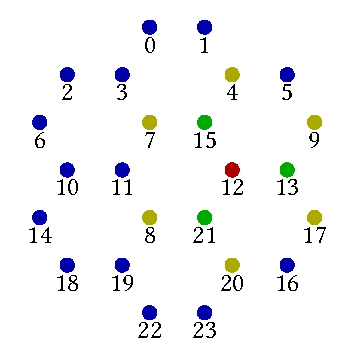
\includegraphics[width=0.3\textwidth]{./theory/physics/explored-lattice-patterns/hexagonal,size=2,np,rs=2.pdf}
    }
    \makebox[\textwidth][c]{
        \includegraphics[width=0.3\textwidth]{./theory/physics/explored-lattice-patterns/trigonal_square,size=3,np.pdf}
        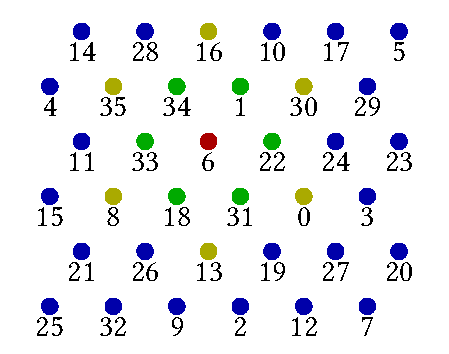
\includegraphics[width=0.3\textwidth]{./theory/physics/explored-lattice-patterns/trigonal_square,size=3,np,rs=-1.pdf}
    }

    \vspace{0.2cm}
    \caption{Visualization of the property \emph{random swaps} of the lattice structure helper. In the first set of figures, two swaps were performed on a hexagonal lattice of size 2 (8 with 15 and 16 with 21). The neighbor-index calculation takes this into effect, therefore the highlighted lattice sites do not change. The second set of figures shows the setting -1 for a trigonal\_square lattice of size 3. This basically makes the generator perform such a high number of pair swaps, that the index-position correlation can be assumed to be random. 
    }
    \label{fig:direct-comparison-lattice-site-swaps}
\end{figure}

The goal of this setting is to decouple the in-memory representation and the structure of the simulated lattice. 
Effects of this will be explored in \fullref{sec:experiments-resiliencylatticeencoding}.

General data about the lattices is provided in \autoref{table:lattice-information}.

\begin{table}[htbp]
    \centering
    \begin{tabular}{l|cc|ccccccc} 
        \toprule
        Lattice name & \#nn & \#nnn &$L$(1)&$L$(2)&$L$(3)&$L$(4)&$L$(5)&$L$(6)&$L$(7)\\  
        \midrule 
        linear & 2 & 2 & 1 & 2 & 3 & 4 & 5 & 6 & 7\\
        cubic & 4 & 4 & 4 & 9 & 16 & 25 & 36 & 49 & 64\\
        trigonal\_square & 6 & 6 & 4 & 16 & 36 & 64 & 100 & 144 & 196\\
        trigonal\_diamond & 6 & 6 & 4 & 9 & 16 & 25 & 36 & 49 & 64\\
        trigonal\_hexagonal & 6 & 6 & 7 & 19 & 37 & 61 & 91 & 127 & 169\\
        hexagonal & 3 & 6 & 6 & 24 & 54 & 96 & 150 & 216 & 294\\
        \bottomrule
    \end{tabular}
    \vspace{0.5cm}
    \caption{General information about the explored lattices. \textbf{\#nn} describes the number of nearest neighbors, \textbf{\#nnn} the number of next nearest neighbors. The numbers describe the maximum possible neighbor count. If a lattice is non-periodic, some sites can have less neighbors. $L(i)$ describes the number of lattice sites for a lattice of \textbf{size=$i$}}.
    \label{table:lattice-information}
\end{table}





        \FloatBarrier
    \section{From the Point of Computer Science}
        \label{sec:theory-cs}
        The first set of experiments will be on the image classification task.
The goal will be to compare the architectural advantages and drawbacks between multiple different kinds of metaformers.

Training was be performed on a subset of 100 classes from the \emph{ImageNet} dataset \cite{imagenetDataset}.
The accompanying code to replicate these experiments can be found on GitHub \cite{selfComputerScience}.

The neural networks, as well as the training and evaluation code were written in python.
The \emph{PyTorch} \cite{pytorchGithub} machine learning framework was used as a measure to efficiently define neural networks and lever the computational capabilities of parallelization via GPUs.

The main metaformer model was originally based on the vision transformer found in an implementation of \emph{DINO} \cite{dinoGithub}, was however heavily modified. 
A comparison between the stock DINO model and the modified version will be also performed.
This however is not supposed to be a direct discrediting of any of the models, as their main purposes do not exactly align.
Therefore one or the other may excel in specific tasks.
Also a comparison against a pre-implemented \emph{poolformer} \cite{poolformerGithub} will be performed.

The \emph{einops} package \cite{einopsGithub} is heavily used. It provides tensor operations, configurable with the \emph{Einstein notation} and simplifies the notation and subsequently readability.
Lastly, the implementation of the \emph{positional encoding} is provided by \cite{positionalEncodingGithub}.

        \FloatBarrier
        \subsection{The Image Classification Task}
        \label{sec:theory-imageclassification}
        \subsection{Neural Network Training}
        \label{sec:theory-neuralnetworktraining}
        \subsection{Neural Network Pre-Training}
        \label{sec:theory-pretraining}
        \subsection{Employment of Graphs for Problem transfer}
        \label{sec:theory-graphs}

\chapter{Machine Learning Architectures}
\label{sec:architectures}

    \section{Used Architectures}
        \subsection{Perceptron Architectures}
        \label{sec:architectures-perceptron}
        \subsection{Pooling}
        \label{sec:architectures-pooling}
        \subsection{Convolutional Architectures}
        \label{sec:architectures-convolution}
        \subsection{Attention and the Transformer}
        \label{sec:architectures-attention}
        \subsection{The Metaformer}
        \label{sec:architectures-metaformer}
        \subsection{Graph Architectures}
        \label{sec:architectures-graphs}
    \section{Usage of Inductive Biases}
        \subsection{Conventional Architectures}
        \label{sec:architectures-biasesnormal}
        \subsection{Metaformer Architectures}
        \label{sec:architectures-biasesmetaformer}
        \subsection{Graph Architectures}
        \label{sec:architectures-biasesgraph}

\chapter{Experiments and their Results}
    \section{Metaformer in Image Classification}
        \subsection{Training Settings}
        \label{sec:experiments-trainingsettings}

        \subsection{Importance of Positional Encoding}
        \label{sec:experiments-positionalencoding}
        \subsection{Comparison of different Token Mixers}
        \label{sec:experiments-tokenmixers}

    \section{Metaformer in Ground State Search}
        \subsection{Comparison to established Architectures}
        \label{sec:experiments-comparisontoestablished}
        \subsection{Resiliency to the Choice of Lattice Encoding}
        \label{sec:experiments-resiliencylatticeencoding}
        \subsection{Optimizing the Ansatz}
        \label{sec:experiments-optimizingtheansatz}
        \subsection{Choice of Hyperparameters}
        \label{sec:experiments-hyperparameters}
        \subsection{Differences across the Phase Diagram}
        \label{sec:experiments-phasecriticalpoint}

\chapter{Conclusion}
\label{sec:conclusion}

% ! Addendum
\newpage
\nocite{*}
\printbibliography[title={Bibliography}]
\chapter{Appendix}
\label{sec:appendix}

%! needs to be first, because of format adapted to chapter title of appendix
\section{Lattice Visualization} \label{appendix:lattice-visualisation}

\begin{minipage}{\linewidth}
    \centering
    \makebox[\textwidth][c]{
        \makebox[1.25\textwidth][c]{
            \makebox[0.40\textwidth][l]{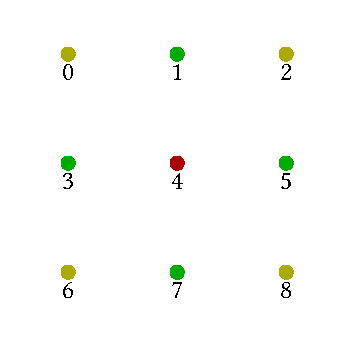
\includegraphics[width=0.33\textwidth]{./../appendix/lattice_visualization/square,size=2,np.pdf}}
            \makebox[0.40\textwidth][l]{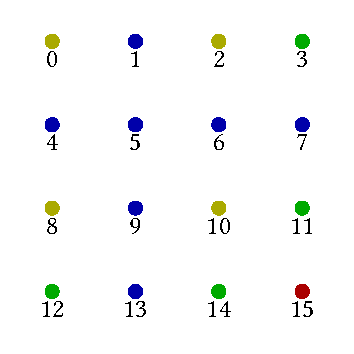
\includegraphics[width=0.33\textwidth]{./../appendix/lattice_visualization/square,size=3,p.pdf}}
            \makebox[0.40\textwidth][l]{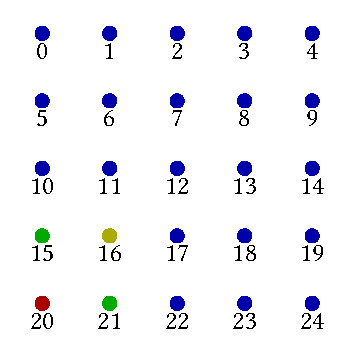
\includegraphics[width=0.33\textwidth]{./../appendix/lattice_visualization/square,size=4,np.pdf}}
        }
    }

    \captionof{figure}{A visualization of the \textbf{2D-square} lattice structure, measured in this thesis. 
        The lattices from left to right can be described by the parameters\\
        1: \emph{size=2, non-periodic}\,\,\,\, 2: \emph{size=3, periodic}\,\,\,\, 3: \emph{size=4, non-periodic}
    }
    \label{fig:appendix-square-lattices}
\end{minipage}

\vspace{0.5cm}

\begin{minipage}{\linewidth}
    \centering
    \makebox[\textwidth][c]{
        \makebox[1.25\textwidth][c]{
            \makebox[0.40\textwidth][l]{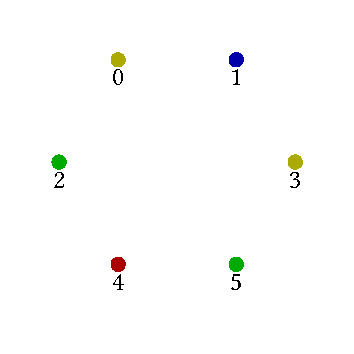
\includegraphics[width=0.33\textwidth]{./../appendix/lattice_visualization/hexagonal,size=1,np.pdf}}
            \makebox[0.40\textwidth][l]{\includegraphics[width=0.33\textwidth]{./../appendix/lattice_visualization/hexagonal,size=2,np.pdf}}
            \makebox[0.40\textwidth][l]{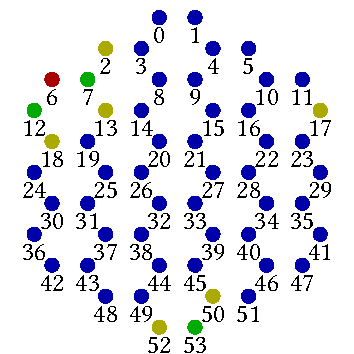
\includegraphics[width=0.33\textwidth]{./../appendix/lattice_visualization/hexagonal,size=3,p.pdf}}
        }
    }

    \vspace{0.3cm}
    \captionof{figure}{A visualization of the \textbf{2D-hexagonal} lattice structure, measured in this thesis. 
        The lattices from left to right can be described by the parameters \\
        1: \emph{size=1, non-periodic}\,\,\,\, 2: \emph{size=2, non-periodic}\,\,\,\, 3: \emph{size=3, periodic}
    }
    \label{fig:appendix-hexagonal-lattices}
\end{minipage}

\vspace{0.4cm}

\begin{minipage}{\linewidth}
    \centering
    \makebox[\textwidth][c]{
        \makebox[1.25\textwidth][c]{
            \makebox[0.40\textwidth][l]{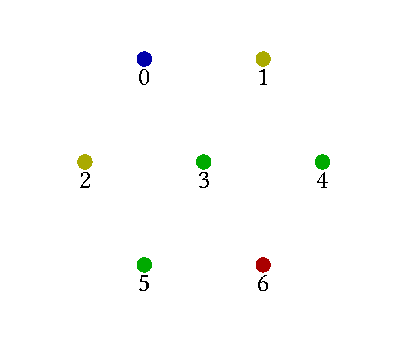
\includegraphics[width=0.33\textwidth]{./../appendix/lattice_visualization/trigonal_hexagonal,size=1,np.pdf}}
            \makebox[0.40\textwidth][l]{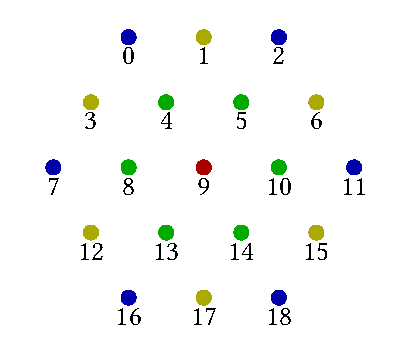
\includegraphics[width=0.33\textwidth]{./../appendix/lattice_visualization/trigonal_hexagonal,size=2,np.pdf}}
            \makebox[0.40\textwidth][l]{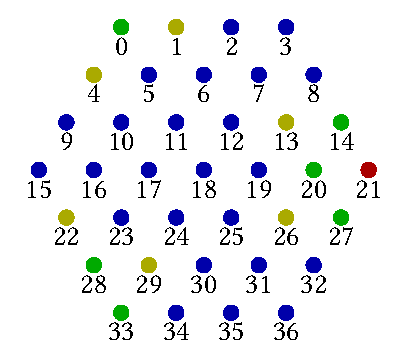
\includegraphics[width=0.33\textwidth]{./../appendix/lattice_visualization/trigonal_hexagonal,size=3,p.pdf}}
        }
    }
    
    \vspace{0.5cm}
    \captionof{figure}{A visualization of the \textbf{2D-trigonal\_hexagonal} lattice structure, measured in this thesis. 
        The lattices from left to right can be described by the parameters \\
        1: \emph{size=1, non-periodic}\,\,\,\, 2: \emph{size=2, non-periodic}\,\,\,\, 3: \emph{size=3, periodic}
    }
    \label{fig:appendix-trigonal_hexagonal-lattices}
\end{minipage}

% HERE SHOULD THE PAGE-BREAK BE. i love latex, but stuff like this infuriates me to get correct
\newpage
\makebox{\vspace{5cm}}\\

\begin{minipage}{\linewidth}
    \centering
    \makebox[\textwidth][c]{
        \makebox[1.25\textwidth][c]{
            \makebox[0.40\textwidth][l]{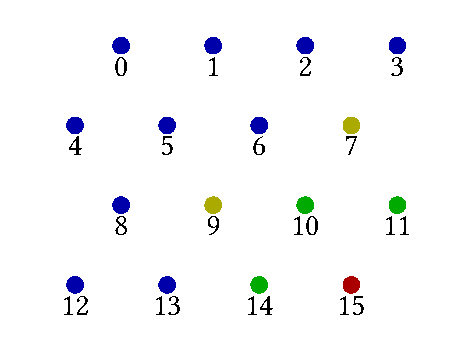
\includegraphics[width=0.33\textwidth]{./../appendix/lattice_visualization/trigonal_square,size=2,np.pdf}}
            \makebox[0.40\textwidth][l]{\includegraphics[width=0.33\textwidth]{./../appendix/lattice_visualization/trigonal_square,size=3,np.pdf}}
            \makebox[0.40\textwidth][l]{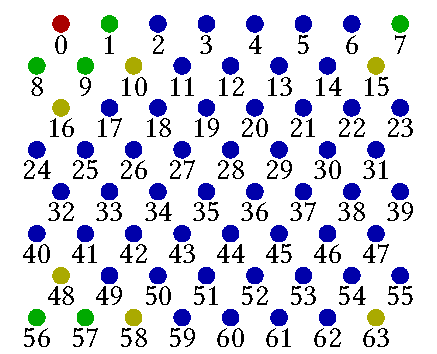
\includegraphics[width=0.33\textwidth]{./../appendix/lattice_visualization/trigonal_square,size=4,p.pdf}}
        }
    }

    \vspace{0.4cm}
    \captionof{figure}{A visualization of the \textbf{2D-trigonal\_square} lattice structure, measured in this thesis. 
        The lattices from left to right can be described by the parameters \\
        1: \emph{size=2, non-periodic}\,\,\,\, 2: \emph{size=3, non-periodic}\,\,\,\, 3: \emph{size=4, periodic}
    }
    \label{fig:appendix-trigonal_square-lattices}
\end{minipage}

\vspace{1.2cm}

\begin{minipage}{\linewidth}
    \centering
    \makebox[\textwidth][c]{
        \makebox[1.25\textwidth][c]{
            \makebox[0.40\textwidth][c]{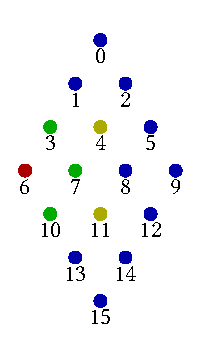
\includegraphics[width=0.20\textwidth]{./../appendix/lattice_visualization/trigonal_diamond,size=3,np.pdf}}
            \makebox[0.40\textwidth][c]{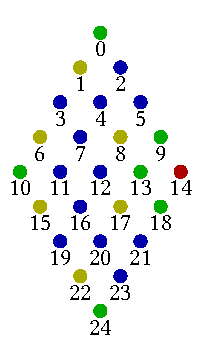
\includegraphics[width=0.20\textwidth]{./../appendix/lattice_visualization/trigonal_diamond,size=4,p.pdf}}
            \makebox[0.40\textwidth][c]{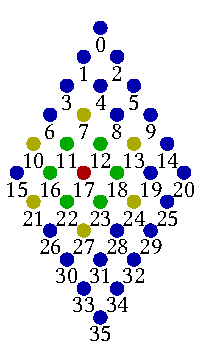
\includegraphics[width=0.20\textwidth]{./../appendix/lattice_visualization/trigonal_diamond,size=5,np.pdf}}
        }
    }

    \vspace{0.4cm}
    \captionof{figure}{A visualization of the \textbf{2D-trigonal\_diamond} lattice structure, measured in this thesis. 
        The lattices from left to right can be described by the parameters \\
        1: \emph{size=3, non-periodic}\,\,\,\, 2: \emph{size=4, periodic}\,\,\,\, 3: \emph{size=5, non-periodic}
    }
    \label{fig:appendix-trigonal_diamond-lattices}
\end{minipage}

\vspace{1.2cm}

\begin{minipage}{\linewidth}
    \centering
    \makebox[\textwidth][c]{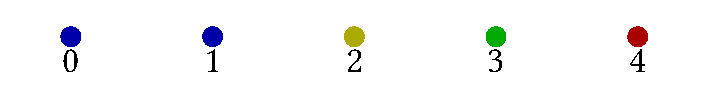
\includegraphics[width=0.80\textwidth]{./../appendix/lattice_visualization/linear,size=5,np.pdf}}
    \vspace*{0.2cm}
    \makebox[\textwidth][c]{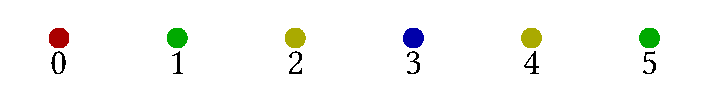
\includegraphics[width=0.80\textwidth]{./../appendix/lattice_visualization/linear,size=6,p.pdf}}
    \vspace*{0.2cm}
    \makebox[\textwidth][c]{
\includegraphics[width=0.80\textwidth]{./../appendix/lattice_visualization/linear,size=8,np.pdf}}

    \vspace{0.2cm}
    \captionof{figure}{A visualization of the \textbf{1D-linear} lattice structure, measured in this thesis. 
        The lattices from top to bottom can be described by the parameters \\
        1: \emph{size=5, non-periodic}\,\,\,\, 2: \emph{size=6, periodic}\,\,\,\, 3: \emph{size=8, non-periodic}
    }
    \label{fig:appendix-linear-lattices}
\end{minipage}

\newpage

% pdf as a additional information, can be nicely ref-ed ("\fullpage{anhang:test}") because of fake section that doesn't get shown in the table of contents
% \includepdf[pagecommand={\section*{} \label{appendix:test}}]{appendix/test.pdf}

% minted to properly import and style code. ! Needs python libraries
\newpage
\section{Dot Product Self Attention (jax)} \label{appendix:attention}
    \cite{selfPhysics}, \filepath{/models/metaformer.py}
    \inputminted[firstline=149, lastline=169]{python}{./../physics-code/models/metaformer.py}

\section{Graph Conformer Module (jax)} \label{appendix:graph-conformer}
    \cite{selfPhysics}, \filepath{/models/metaformer.py}
    \inputminted[firstline=242, lastline=284]{python}{./../physics-code/models/metaformer.py}

\newpage
\section{Graph Poolformer Module (jax)} \label{appendix:graph-poolformer}
    \cite{selfPhysics}, \filepath{/models/metaformer.py}
    \inputminted[firstline=211, lastline=239]{python}{./../physics-code/models/metaformer.py}
    

\end{document}





